\documentclass[12pt, letterpaper]{article}
\usepackage{graphicx} % Required for inserting images
\usepackage{amssymb}
\usepackage{tkz-graph}
\usepackage{float}
\usepackage{subcaption}

\title{Proof of some Graph Invariants 

(Order and Size)}
\author{Wich Moonsarn\\Special Mathematics Lecture (Graph Theory)\\Nagoya University, Spring 2024}
\date{}

\begin{document}
\maketitle
To avoid misunderstanding, we first provide some related definitions at the beginning of this report. Then, The Main objective of this report is to show that that order and the size are graph invariants.

\textbf{Definition 1} (Order and Size). For a finite graph $G = (V, E)$, the \textit{Order} of $G$ ($\vert G \vert$) is the number of element in the set $V$ and the \textit{Size} of $G$ ($\vert\vert G \vert\vert$) is the number of element in the set $E$.

\textbf{Definition 2} (Isomorphism of graph). Let $G = (V, E, i)$ and $G' = (V', E', i')$ be two graphs. A map $f : G \rightarrow G'$ is an \textit{isomorphism of graphs} if $f = (f_V, f_E)$ with $f_V : V \rightarrow V'$ and $f_E : E \rightarrow E'$ satisfy
\begin{enumerate}
  \item $f_V$ and $f_E$ are bijective functions.
  \item $\forall e \in E$ with $i(e) = (x, y)$ in $V \times V$, one has $i'(f_E(e)) = (f_V(x), f_V(y))$ in $V' \times V'$.
\end{enumerate}

\textbf{Definition 3} (Graph invariant). A \textit{Graph invariant} is a property of the graph which is preserved by isomorphism.

\textbf{Proposition 4} (Graph invariant 1). The order and the size are graph invariants.

\textit{Proof} Let $f = (f_V, f_E)$ with $f_V : V \rightarrow V'$ and $f_E : E \rightarrow E'$ be isomorphism of graph between $G = (V, E, i)$ and $G' = (V', E', i')$. 

$f_V$ is injective, $\forall v_1, v_2 \in V, v_1 \neq v_2 \Rightarrow f_V(v_1) \neq f_V(v_2)$ (different element in $V$ cannot be mapped with the same element in $V'$). So, $\vert G \vert \leq \vert G' \vert$.

$f_E$ is injective, $\forall e_1, e_2 \in E, e_1 \neq e_2 \Rightarrow f_E(e_1) \neq f_E(e_2)$ (different element in $E$ cannot be mapped with the same element in $E'$). So, $\vert\vert G \vert\vert \leq \vert\vert G' \vert\vert$.

$f_V$ is surjective, $\forall v' \in V', \exists v \in V$ such that $v' = f_V(v)$ (All element in $V'$ are image of some element in $V$). So, $\vert G \vert \geq \vert G' \vert$.

$f_E$ is surjective, $\forall e' \in E', \exists e \in E$ such that $e' = f_E(e)$ (All element in $E'$ are image of some element in $E$). So, $\vert\vert G \vert\vert \geq \vert\vert G' \vert\vert$.

From $\vert G \vert \leq \vert G' \vert$ and $\vert G \vert \geq \vert G' \vert$, It can emphasizes that $\vert G \vert = \vert G' \vert$.

From $\vert\vert G \vert\vert \leq \vert\vert G' \vert\vert$ and $\vert\vert G \vert\vert \geq \vert\vert G' \vert\vert$, It can emphasizes that $\vert\vert G \vert\vert = \vert\vert G' \vert\vert$.

$\therefore$ The order and the size are graph invariants.

Considering about converse of this proposition, in other word “If two graphs have the same order and the same size, then they are isomorphic". We can find some counterexample shown in figure \ref{fig:entire_fig} below.

\begin{figure}[H]
\begin{subfigure}{0.4\textwidth}
    \centering
    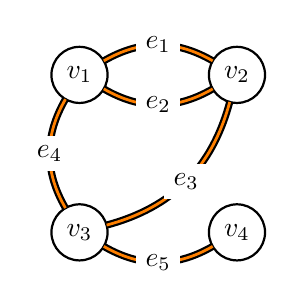
\begin{tikzpicture}
    \GraphInit[vstyle=Shade]
    \tikzset{VertexStyle/.style = {draw, thick, circle, fill=white}}
    \SetGraphUnit{2}
    \Vertex[Math] {v_3}
    \EA[Math](v_3){v_4}
    \SetGraphUnit{2}
    \NO[Math](v_3){v_1}
    \EA[Math](v_1){v_2}
    \tikzset{EdgeStyle/.append style = {bend left}}
    \Edge[label=$e_1$](v_1)(v_2)
    \Edge[label=$e_2$](v_2)(v_1)
    \Edge[label=$e_3$](v_2)(v_3)
    \tikzset{EdgeStyle/.append style = {bend right}}
    \Edge[label=$e_4$](v_1)(v_3)
    \Edge[label=$e_5$](v_3)(v_4)
    \end{tikzpicture}
    \caption{Graph $G$}
    \label{fig:subfig_a}
\end{subfigure}
\hfill
\begin{subfigure}{0.4\textwidth}
    \centering
    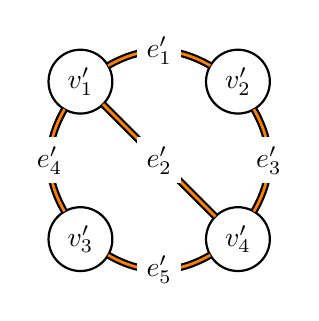
\begin{tikzpicture}
    \GraphInit[vstyle=Shade]
    \tikzset{VertexStyle/.style = {draw, thick, circle, fill=white}}
    \SetGraphUnit{2}
    \Vertex[Math] {v'_3}
    \EA[Math](v'_3){v'_4}
    \SetGraphUnit{2}
    \NO[Math](v'_3){v'_1}
    \EA[Math](v'_1){v'_2}
    \Edge[label=$e'_2$](v'_1)(v'_4)
    \tikzset{EdgeStyle/.append style = {bend left}}
    \Edge[label=$e'_1$](v'_1)(v'_2)
    \Edge[label=$e'_3$](v'_2)(v'_4)
    \tikzset{EdgeStyle/.append style = {bend right}}
    \Edge[label=$e'_4$](v'_1)(v'_3)
    \Edge[label=$e'_5$](v'_3)(v'_4)
    \end{tikzpicture}
    \caption{Graph $G'$}
    \label{fig:subfig_b}
\end{subfigure}
\caption{Two graphs with the same order and size}
\label{fig:entire_fig}
\end{figure}

Graph $G$ has 4 vertices and 5 edges, same number with graph $G'$, and we can obviously see that they are not isomorphic. So, this statement, converse of this proposition, is false.

\end{document}